\documentclass[14pt]{extreport}
\usepackage{gost}

\begin{document}

\pagestyle{empty}
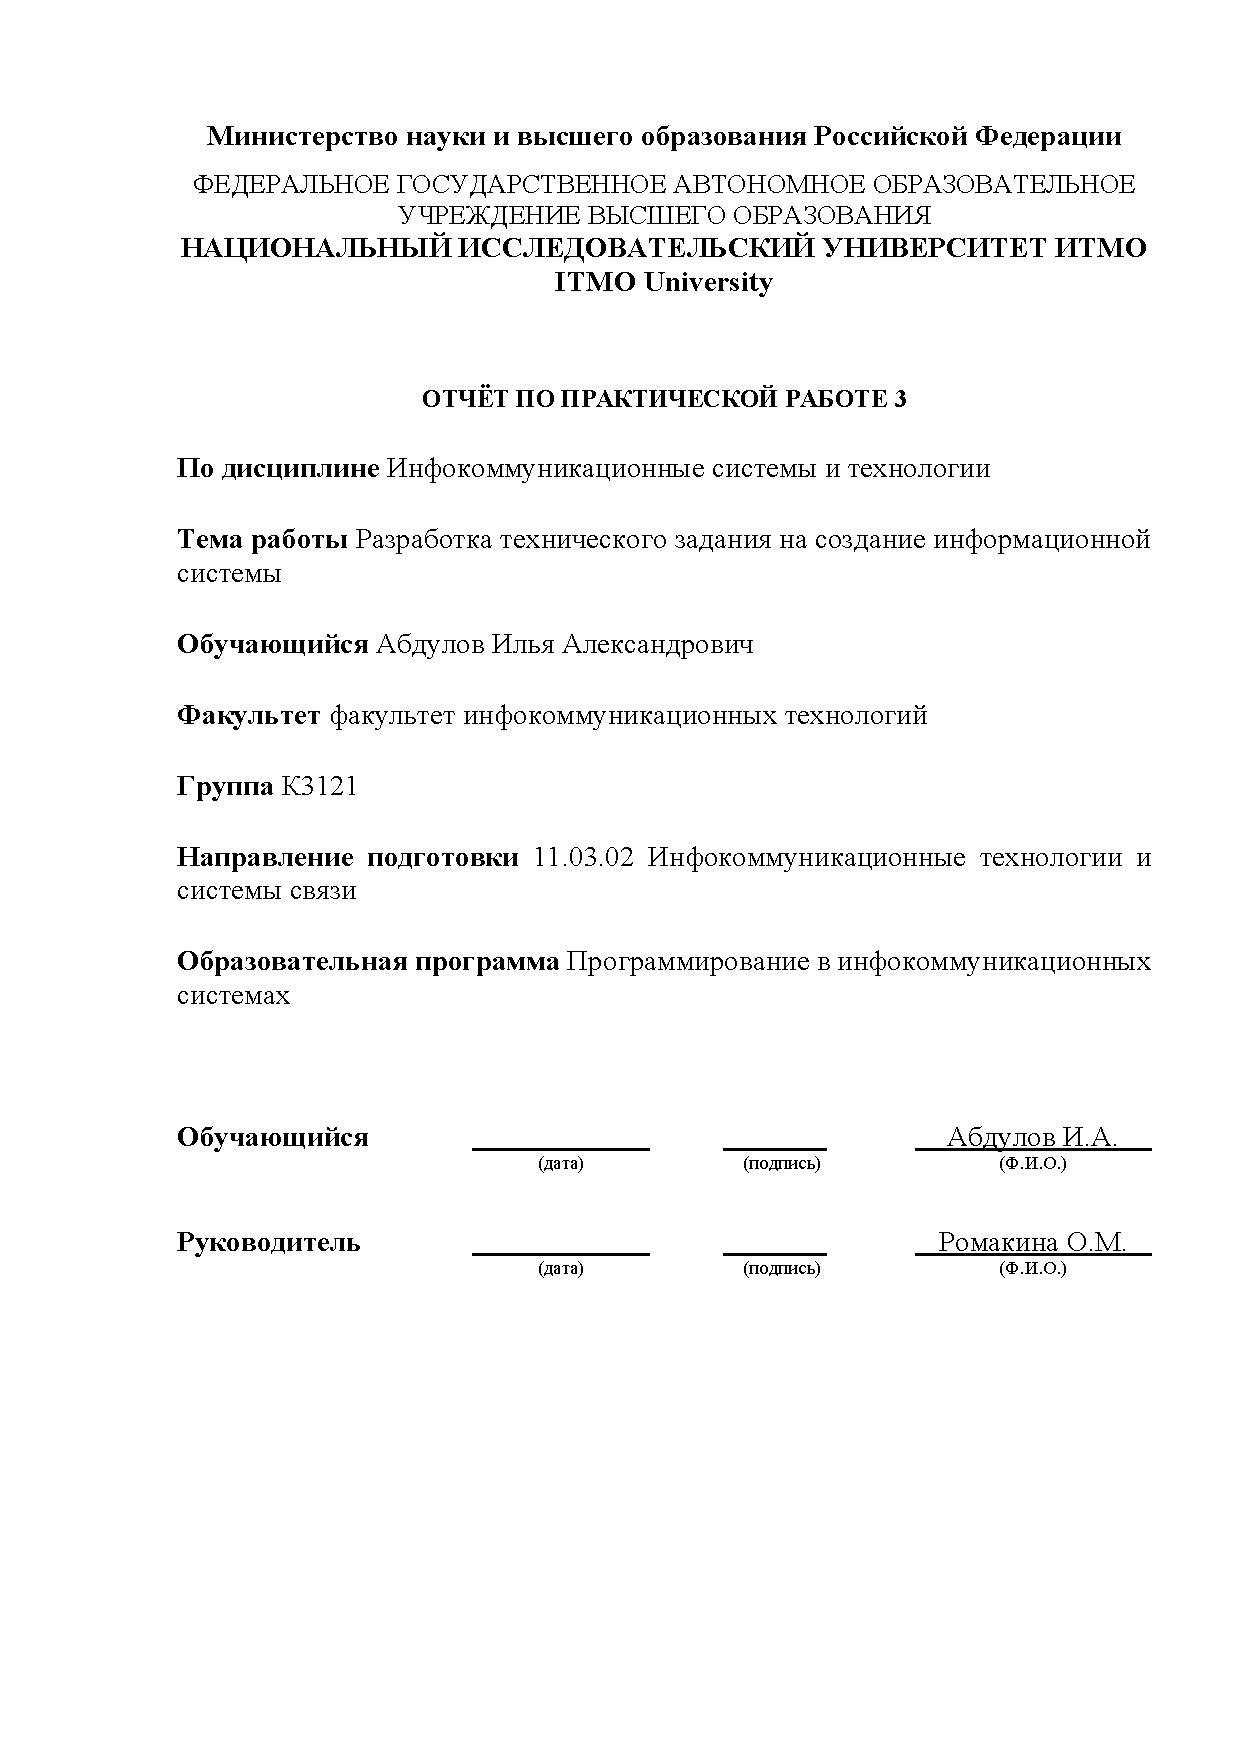
\includepdf{titulCourse.pdf}
\pagestyle{plain}

\tableofcontents

\intro

Данная работа представляет собой отчет о выполненных заданиях:
\begin{enumerate}
\item Написать программу с функциями для быстрой сортировки и сортировки расческой. Использовать данные функции п программу как модуль в другой программе. Пользователь выбирает один из двух методов сортировки. Оценить время выполнения программы с помощью модуля timeit.
\item Изучить блочную и пирамидальную сортировку. Написать соответствующие программы.
\item Оцените достоинства, недостатки и сложность изученных методов сортировок.
\end{enumerate}

\chapter{Задание 1}

Быстрая сортировка заключается в том, что массив делится на две части относительно опорного элемента. В одну часть помещаются все элементы, величина которых меньше значения опорного элемента, а в правую часть — элементы со значением больше опорного. Таким образом каждая из частей так же рекурсивно делится на две части, результатом сортировки является слияние списков, возвращаемых рекурсией.

\begin{figure}[H]
\centerline{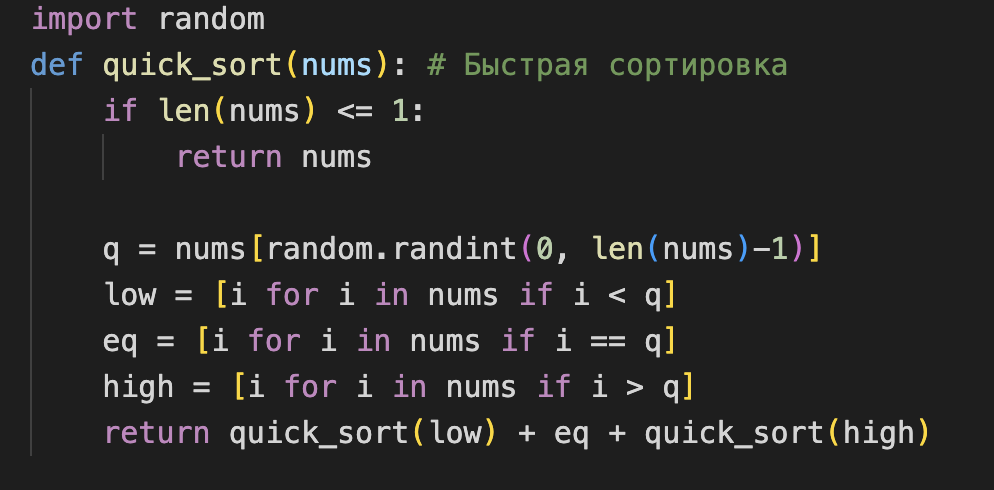
\includegraphics[width=0.7\linewidth]{QuickSort.png}}
\caption{Код функции для быстрой сортировки}
\label{fig11}
\end{figure}

Сортировка расческой заключается в том, чтобы “устранить” элементы с небольшими значениями в конце массива, которые замедляют работу алгоритма. При этой сортировке сначала берется большое расстояние между сравниваемыми значениями, а потом оно сужается вплоть до минимального.

\begin{figure}[H]
\centerline{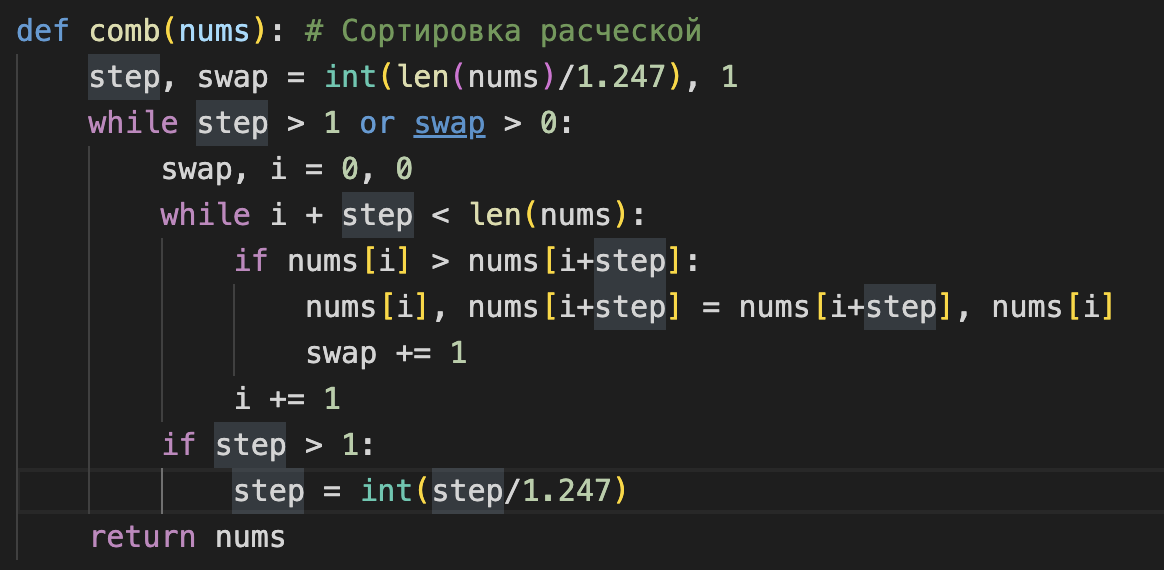
\includegraphics[width=0.7\linewidth]{Comb.png}}
\caption{Код функции для сортировки расческой}
\label{fig12}
\end{figure}

Используем две данные функции сортировки как модуль в другой программе.

\begin{figure}[H]
\centerline{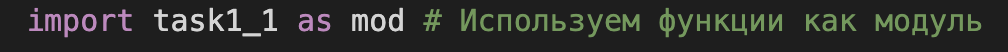
\includegraphics[width=0.7\linewidth]{Mod.png}}
\caption{Код импорта функций из другой программы}
\label{fig13}
\end{figure}

Рассмотрим процесс работы программы, в которой пользователь выбирает разные методы сортировки.

\begin{figure}[H]
\centerline{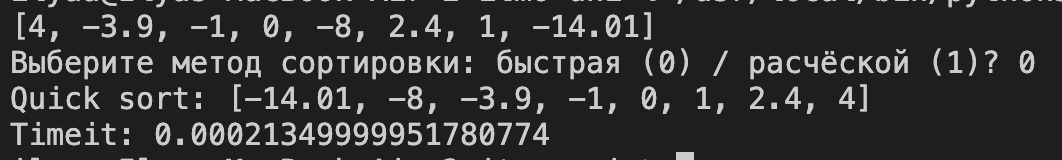
\includegraphics[width=0.7\linewidth]{Example1.png}}
\caption{Пример работы быстрой сортировки}
\label{fig14}
\end{figure}

\begin{figure}[H]
\centerline{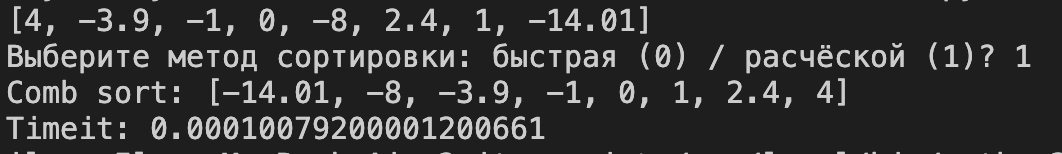
\includegraphics[width=0.7\linewidth]{Example2.png}}
\caption{Пример работы сортировки расческой}
\label{fig15}
\end{figure}

Вывод: быстрая сортировка является одним из наиболее эффективных методов упорядочивания данных. На больших массивах данных сортировка расческой менее эффективна, чем быстрая, но на маленьких, как и показал пример, работает в несколько раз быстрее.

\chapter{Задание 2}

Блочная сортировка заключается в том, чтобы распределить элементы между конечным числом отдельных блоков так, чтобы все элементы в каждом следующем по порядку блоке были всегда больше, чем в предыдущем. Каждый блок затем сортируется отдельно. Отсортированные элементы помещаются обратно в массив.

\begin{figure}[H]
\centerline{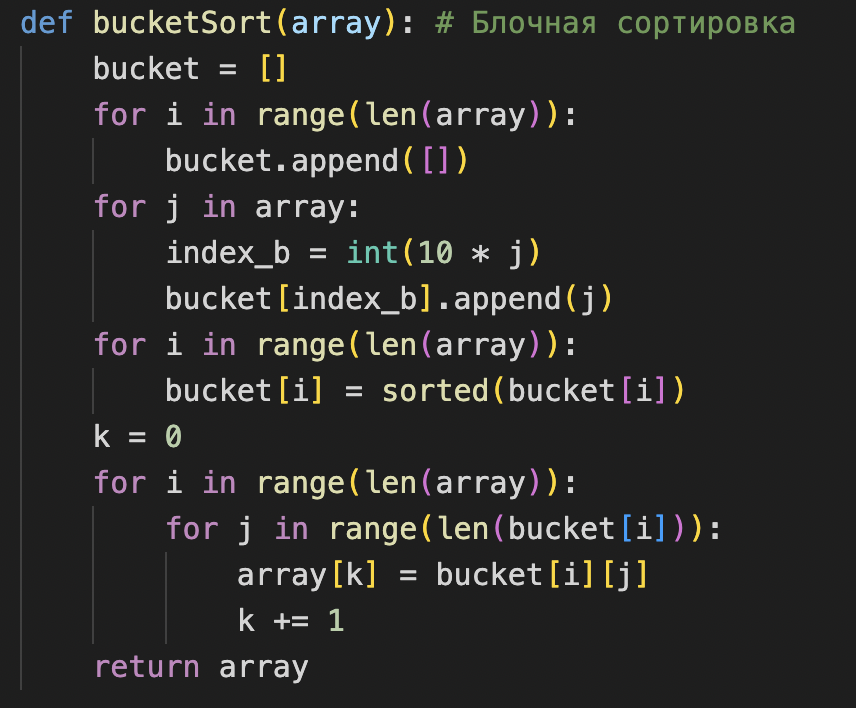
\includegraphics[width=0.59\linewidth]{BucketSort.png}}
\caption{Код функции блочной сортировки}
\label{fig16}
\end{figure}

Пирамидальная сортировка является усовершенствованной сортировкой пузырьком, в которой элемент всплывает / тонет по путям бинарного дерева.

\begin{figure}[H]
\centerline{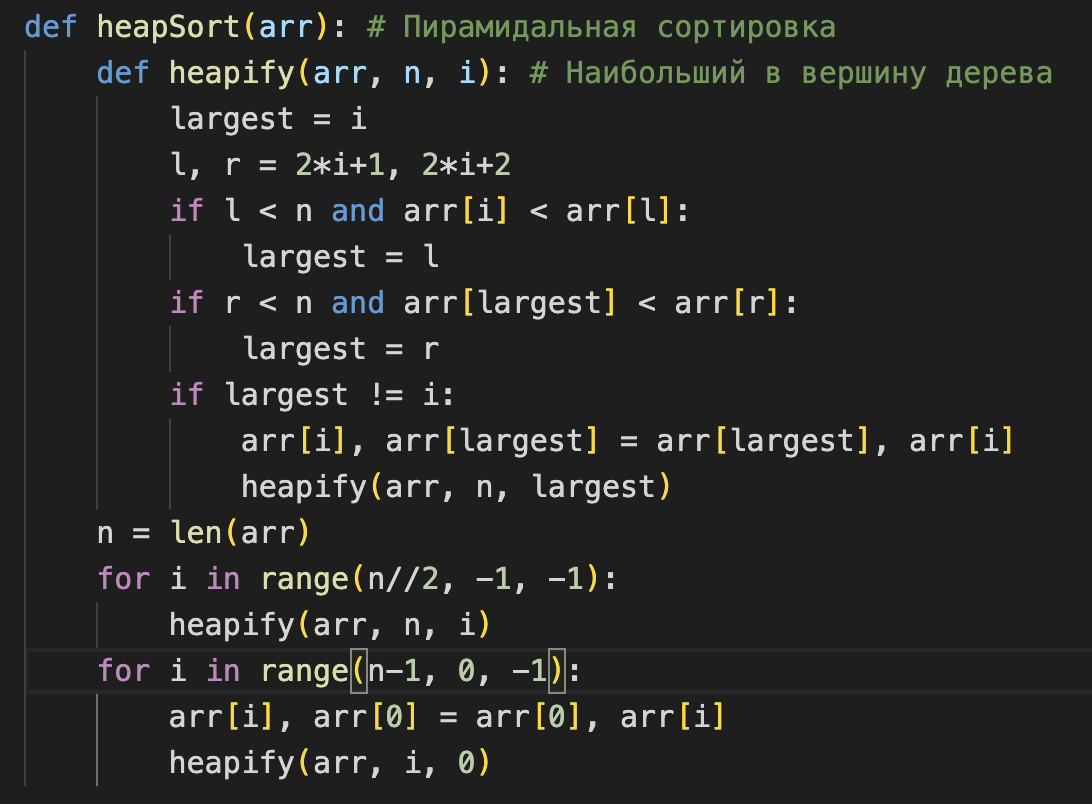
\includegraphics[width=0.59\linewidth]{HeapSort.png}}
\caption{Код функции пирамидальной сортировки}
\label{fig17}
\end{figure}

\chapter{Задание 3}

Алгоритм быстрой сортировки является одним из лучших и наиболее эффективных алгоритмов сортировки, а его рекурсивная реализация очень проста. К недостаткам можно отнести неустойчивость и деградацию скорости в худшем из случаев входных данных. Сложность $O(n^2)$.

Сортировка расческой является довольно упрощённым алгоритмом упорядочивания, улучшает сортировку пузырьком. В лучшем случае алгоритм имеет сложность $O(n\log 2n)$, в худшем случае работает за экспоненциальное $O(n^2)$ время.

Блочный тип сортировки может обладать линейным $O(n)$ временем исполнения на удачных входных данных. В худшем случае будет иметь экспоненциальное $O(n^2)$ время работы. Алгоритм применим к элементам, которые равномерно распределены.

Пирамидальная сортировка в среднем работает очень быстро, но на почти отсортированных массивах работает столь же долго, как и на хаотических данных. Зато, алгоритм эффективен по памяти, так как сортирует элементы на месте. Сложность алгоритма $O(n\log n)$

\conclusions

Таким образом, для каждой задачи была написана программа на языке программирования Python. Были изучены 4 алгоритма сортировки массива и рассмотрены их достоинства, недостатки и сложность. Для каждого алгоритма приведены программы.

Все программы можно найти на репозитории в GitHub\cite{bib1}.

\newpage
\begin{thebibliography}{99}

\bibitem{bib1}GitHub [Электронный ресурс]: \url{https://github.com/estle/itmo-uni/tree/main/sem1/ADS/lab4} (дата обращения 02.12.2022).

\end{thebibliography}

\end{document}
